\subsection{Bedienung}
{\large Quellen und Referenzen verwalten, jetzt neu bequem in JavaFX.\\}

Übersichtsfenster über den Menüpunkt View wechselbar.\\
Einträge über den Menüpunkt Edit verwalten oder bequemer mit den Schnelltasten:
\begin{itemize}
	\item Doppelklick oder Enter auf existierendem Objekt: Gewähltes Objekt bearbeiten.
	\item Doppelklick auf leere Zeile: Neues Objekt erstellen.
	\item Delete: Gewähltes Objekt löschen.
\end{itemize}

\begin{figure}[H]
	\centering
	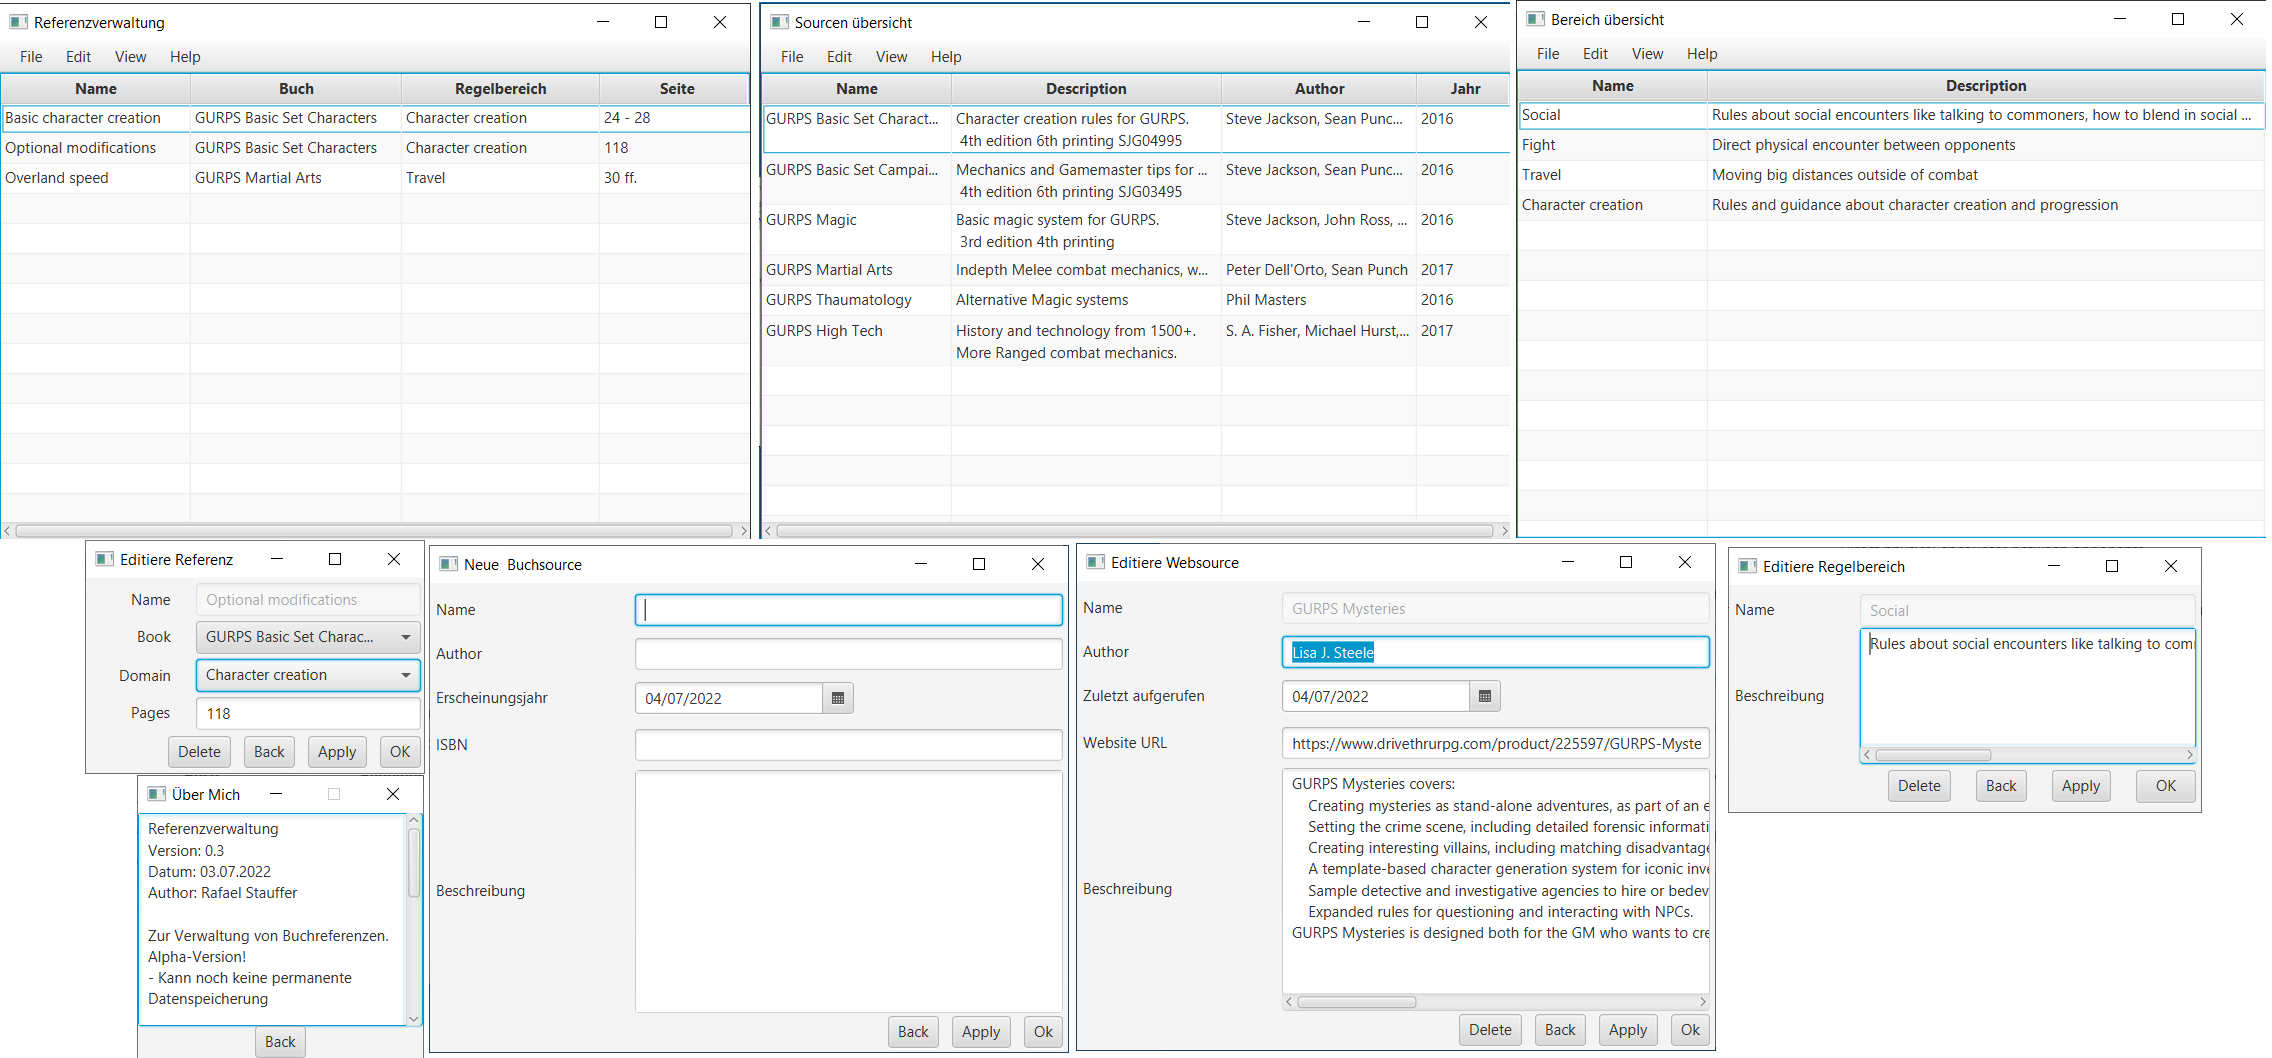
\includegraphics[width=0.95\textwidth]{screenshots}
	\caption{Alle Fenster im Überblick.\\{\footnotesize Von links oben im Uhrzeigersinn: Referenzübersicht-Hauptfenster, Sourcenübersicht, Bereichsübersicht, Bereich-Detailfenster im Editiermodus, Website-Detailfenster im Editiermodus, Buch-Detailfenster im Erstellmodus, ÜberMich-Infofenster, Referenz-Detailfenster im Editiermodus}}
\end{figure}

\subsection{Git}

Das Projekt ist unter \url{https://dev.hftm.ch:4430/rafael.stauffer/oop1-projektarbeit} gespeichert.\\
Wie im ReadMe beschreiben kann das maven verzeichnis per {\ttfamily mvn clean javafx:run} direkt ausgeführt oder per {\ttfamily mvn clean compile package} in ein JAR kompiliert werden welches sich unter {\ttfamily /maven/target/Referenzverwaltung-0.3-SNAPSHOT.jar} befindet.

\subsection{Code Architektur}

Im total existieren acht Controller-Klassen mit je einer dazugehörigen View welche von der BaseController-Basisklasse abgelietet werden.
Die drei Overview-Klassen sind für die jeweiligen Tabellenübersichten zuständig. Die vier Detail-Klassen verwalten die Erstell- und Bearbeitungs-formulare. Der AboutController verwaltet das ÜberMich-Fenster.

\begin{figure}[H]
	\centering
	
\includegraphics[width=0.95\textwidth]{controller}
	\caption{Controller-Klassen}
\end{figure}

Business-Daten wurden wie im Szenarienbeschrieb definiert in drei Klassen gespeichert, dabei wurde aber die Source-Klasse weiter in SourceBook (mit Erscheinungsjahr und ISBN) und SourceWeb (mit URL und letztem Seitenaufruf) unterteilt.

\begin{figure}[H]
	\centering
	
\includegraphics[width=0.95\textwidth]{business_klassen}
	\caption{Business-Objekte und DataAccessObject}
\end{figure}